\documentclass[ignorenonframetext,]{beamer}
\setbeamertemplate{caption}[numbered]
\setbeamertemplate{caption label separator}{: }
\setbeamercolor{caption name}{fg=normal text.fg}
\beamertemplatenavigationsymbolsempty
\usepackage{lmodern}
\usepackage{amssymb,amsmath}
\usepackage{ifxetex,ifluatex}
\usepackage{fixltx2e} % provides \textsubscript
\ifnum 0\ifxetex 1\fi\ifluatex 1\fi=0 % if pdftex
  \usepackage[T1]{fontenc}
  \usepackage[utf8]{inputenc}
\else % if luatex or xelatex
  \ifxetex
    \usepackage{mathspec}
  \else
    \usepackage{fontspec}
  \fi
  \defaultfontfeatures{Ligatures=TeX,Scale=MatchLowercase}
\fi
\usetheme[]{CambridgeUS}
\usecolortheme{beaver}
\usefonttheme{structurebold}
% use upquote if available, for straight quotes in verbatim environments
\IfFileExists{upquote.sty}{\usepackage{upquote}}{}
% use microtype if available
\IfFileExists{microtype.sty}{%
\usepackage{microtype}
\UseMicrotypeSet[protrusion]{basicmath} % disable protrusion for tt fonts
}{}
\newif\ifbibliography
\hypersetup{
            pdftitle={Geomedizin mit R},
            pdfauthor={Jan-Philipp Kolb},
            pdfborder={0 0 0},
            breaklinks=true}
\urlstyle{same}  % don't use monospace font for urls
\usepackage{color}
\usepackage{fancyvrb}
\newcommand{\VerbBar}{|}
\newcommand{\VERB}{\Verb[commandchars=\\\{\}]}
\DefineVerbatimEnvironment{Highlighting}{Verbatim}{commandchars=\\\{\}}
% Add ',fontsize=\small' for more characters per line
\usepackage{framed}
\definecolor{shadecolor}{RGB}{42,33,28}
\newenvironment{Shaded}{\begin{snugshade}}{\end{snugshade}}
\newcommand{\KeywordTok}[1]{\textcolor[rgb]{0.26,0.66,0.93}{\textbf{#1}}}
\newcommand{\DataTypeTok}[1]{\textcolor[rgb]{0.74,0.68,0.62}{\underline{#1}}}
\newcommand{\DecValTok}[1]{\textcolor[rgb]{0.27,0.67,0.26}{#1}}
\newcommand{\BaseNTok}[1]{\textcolor[rgb]{0.27,0.67,0.26}{#1}}
\newcommand{\FloatTok}[1]{\textcolor[rgb]{0.27,0.67,0.26}{#1}}
\newcommand{\ConstantTok}[1]{\textcolor[rgb]{0.74,0.68,0.62}{#1}}
\newcommand{\CharTok}[1]{\textcolor[rgb]{0.02,0.61,0.04}{#1}}
\newcommand{\SpecialCharTok}[1]{\textcolor[rgb]{0.02,0.61,0.04}{#1}}
\newcommand{\StringTok}[1]{\textcolor[rgb]{0.02,0.61,0.04}{#1}}
\newcommand{\VerbatimStringTok}[1]{\textcolor[rgb]{0.02,0.61,0.04}{#1}}
\newcommand{\SpecialStringTok}[1]{\textcolor[rgb]{0.02,0.61,0.04}{#1}}
\newcommand{\ImportTok}[1]{\textcolor[rgb]{0.74,0.68,0.62}{#1}}
\newcommand{\CommentTok}[1]{\textcolor[rgb]{0.00,0.40,1.00}{\textit{#1}}}
\newcommand{\DocumentationTok}[1]{\textcolor[rgb]{0.00,0.40,1.00}{\textit{#1}}}
\newcommand{\AnnotationTok}[1]{\textcolor[rgb]{0.00,0.40,1.00}{\textbf{\textit{#1}}}}
\newcommand{\CommentVarTok}[1]{\textcolor[rgb]{0.74,0.68,0.62}{#1}}
\newcommand{\OtherTok}[1]{\textcolor[rgb]{0.74,0.68,0.62}{#1}}
\newcommand{\FunctionTok}[1]{\textcolor[rgb]{1.00,0.58,0.35}{\textbf{#1}}}
\newcommand{\VariableTok}[1]{\textcolor[rgb]{0.74,0.68,0.62}{#1}}
\newcommand{\ControlFlowTok}[1]{\textcolor[rgb]{0.26,0.66,0.93}{\textbf{#1}}}
\newcommand{\OperatorTok}[1]{\textcolor[rgb]{0.74,0.68,0.62}{#1}}
\newcommand{\BuiltInTok}[1]{\textcolor[rgb]{0.74,0.68,0.62}{#1}}
\newcommand{\ExtensionTok}[1]{\textcolor[rgb]{0.74,0.68,0.62}{#1}}
\newcommand{\PreprocessorTok}[1]{\textcolor[rgb]{0.74,0.68,0.62}{\textbf{#1}}}
\newcommand{\AttributeTok}[1]{\textcolor[rgb]{0.74,0.68,0.62}{#1}}
\newcommand{\RegionMarkerTok}[1]{\textcolor[rgb]{0.74,0.68,0.62}{#1}}
\newcommand{\InformationTok}[1]{\textcolor[rgb]{0.00,0.40,1.00}{\textbf{\textit{#1}}}}
\newcommand{\WarningTok}[1]{\textcolor[rgb]{1.00,1.00,0.00}{\textbf{#1}}}
\newcommand{\AlertTok}[1]{\textcolor[rgb]{1.00,1.00,0.00}{#1}}
\newcommand{\ErrorTok}[1]{\textcolor[rgb]{1.00,1.00,0.00}{\textbf{#1}}}
\newcommand{\NormalTok}[1]{\textcolor[rgb]{0.74,0.68,0.62}{#1}}
\usepackage{longtable,booktabs}
\usepackage{caption}
% These lines are needed to make table captions work with longtable:
\makeatletter
\def\fnum@table{\tablename~\thetable}
\makeatother
\usepackage{graphicx,grffile}
\makeatletter
\def\maxwidth{\ifdim\Gin@nat@width>\linewidth\linewidth\else\Gin@nat@width\fi}
\def\maxheight{\ifdim\Gin@nat@height>\textheight0.8\textheight\else\Gin@nat@height\fi}
\makeatother
% Scale images if necessary, so that they will not overflow the page
% margins by default, and it is still possible to overwrite the defaults
% using explicit options in \includegraphics[width, height, ...]{}
\setkeys{Gin}{width=\maxwidth,height=\maxheight,keepaspectratio}

% Prevent slide breaks in the middle of a paragraph:
\widowpenalties 1 10000
\raggedbottom

\AtBeginPart{
  \let\insertpartnumber\relax
  \let\partname\relax
  \frame{\partpage}
}
\AtBeginSection{
  \ifbibliography
  \else
    \let\insertsectionnumber\relax
    \let\sectionname\relax
    \frame{\sectionpage}
  \fi
}
\AtBeginSubsection{
  \let\insertsubsectionnumber\relax
  \let\subsectionname\relax
  \frame{\subsectionpage}
}

\setlength{\parindent}{0pt}
\setlength{\parskip}{6pt plus 2pt minus 1pt}
\setlength{\emergencystretch}{3em}  % prevent overfull lines
\providecommand{\tightlist}{%
  \setlength{\itemsep}{0pt}\setlength{\parskip}{0pt}}
\setcounter{secnumdepth}{0}

\title{Geomedizin mit R}
\author{Jan-Philipp Kolb}
\date{11 Januar 2019}

\begin{document}
\frame{\titlepage}

\begin{frame}{Kleine Vorstellungsrunde}

\begin{itemize}
\tightlist
\item
  Wo kommt Ihr her?
\item
  Wo arbeitet oder studiert Ihr?
\item
  Wie beurteilt Ihr Eure Fähigkeiten mit R?
\item
  Habt Ihr Erfahrungen mit anderen Programmiersprachen /
  Statistiksoftware? Wenn ja welche?
\item
  Was sind Eure Erwartungen für diesen Kurs?
\end{itemize}

\end{frame}

\begin{frame}{Informationen vorab}

Normalerweise gibt es große Unterschiede bei Vorkenntnissen und
Fähigkeiten, insbesondere bei diesem Kurs.

\begin{itemize}
\tightlist
\item
  Bitte gebt Bescheid, wenn es zu schnell oder zu langsam geht oder
  etwas unklar geblieben ist.
\item
  Wenn es Fragen gibt - immer fragen
\item
  Wenn Ihr etwas hinzuzufügen habt - sehr gerne
\item
  In diesem Kurs gibt es viele
  \href{http://web.math.ku.dk/~helle/R-intro/exercises.pdf}{\textbf{Übungen}},
  denn das Programmieren / die Nutzung von Geodaten in R lernt man am
  Ende (wie vieles) nur allein.
\item
  Ich habe viele \href{https://www.showmeshiny.com/}{\textbf{Beispiele}}
  - probiert sie aus
\item
  R macht mehr Spaß zusammen - arbeitet zusammen!
\end{itemize}

\end{frame}

\begin{frame}{Disclaimer}

\begin{itemize}
\tightlist
\item
  Zum Import, zur Verarbeitung und Visualisierung gibt es bereits sehr
  viele Pakete.
\item
  Das Gebiet entwickelt sich sehr schnell.
\item
  Es ist nicht möglich alles davon in diesem Kurs vorzustellen.
\item
  Ich möchte anhand einiger interessanter Beispiele einen Einblick darin
  geben, was alles möglich ist.
\end{itemize}

\end{frame}

\begin{frame}{Disclaimer/ Informationen vorab}

Normalerweise gibt es große Unterschiede bei Vorkenntnissen und
Fähigkeiten - bitte gebt Bescheid, wenn es zu schnell oder zu langsam
geht oder etwas unklar geblieben ist.

\begin{itemize}
\tightlist
\item
  Wenn es Fragen gibt - immer fragen
\item
  In diesem Kurs gibt es viele
  \href{http://web.math.ku.dk/~helle/R-intro/exercises.pdf}{\textbf{Übungen}},
  denn das Programmieren / die Nutzung von R lernt man am Ende nur
  allein.
\item
  Ich habe viele \href{https://www.showmeshiny.com/}{\textbf{Beispiele}}
  - probiert sie aus
\item
  R macht mehr Spaß zusammen - arbeitet zusammen!
\end{itemize}

\end{frame}

\begin{frame}{Gründe R zu nutzen\ldots{}}

\begin{itemize}
\item
  \ldots{} R ist eine
  \href{https://stackoverflow.com/questions/1546583/what-is-the-definition-of-an-open-source-programming-language}{\textbf{quelloffene
  Sprache}}
\item
  \ldots{} hervorragende
  \href{http://matthewlincoln.net/2014/12/20/adjacency-matrix-plots-with-r-and-ggplot2.html}{\textbf{Grafiken}},
  \href{https://www.r-bloggers.com/3d-plots-with-ggplot2-and-plotly\%20/}{\textbf{Grafiken}},
  \href{https://procomun.wordpress.com/2011/03/18/splomr/}{\textbf{Grafiken}}
\item
  \ldots{} \href{https://github.com/Japhilko/RInterfaces}{\textbf{R kann
  in Kombination mit anderen Programmen verwendet werden}} - z.B. zur
  \href{https://github.com/Japhilko/RInterfaces/blob/master/slides/Datenimport.md}{\textbf{Verknüpfung
  von Daten}}
\item
  \ldots{} R kann
  \href{https://cran.r-project.org/web/packages/MplusAutomation/index.html}{\textbf{zur
  Automatisierung}} verwendet werden
\item
  \ldots{} Breite und aktive Community -
  \href{https://www.r-bloggers.com/}{\textbf{Man kann die Intelligenz
  anderer Leute nutzen ;-)}}
\end{itemize}

\end{frame}

\begin{frame}{R kann in Kombination mit anderen Programmen genutzt
werden\ldots{}}

\begin{figure}
\centering

\includegraphics{D:/Daten/GitHub/IntroR/buildingblocks/figure/Rinterfaces.PNG}
\caption{Schnittstellen zu R}
\end{figure}

\begin{itemize}
\tightlist
\item
  Schnittstelle zu:
  \href{https://cran.r-project.org/web/packages/reticulate/vignettes/calling_python.html}{\textbf{Python}},
  \href{https://www.springer.com/de/book/9781441900517}{\textbf{Excel}},
  \href{https://www.ibm.com/support/knowledgecenter/en/SSFUEU_7.2.0/com.ibm.swg.ba.cognos.op_capmod_ig.7.2.0.doc/t_essentials_for_r_statistics.html}{\textbf{SPSS}},
  \href{https://cran.r-project.org/web/packages/SASmixed/index.html}{\textbf{SAS}},
  \href{https://cran.r-project.org/web/packages/RStata/index.html}{\textbf{Stata}}
\end{itemize}

\end{frame}

\begin{frame}{\href{https://gallery.shinyapps.io/cran-gauge/}{\textbf{Die
Beliebtheit von R-Paketen}}}

\begin{figure}
\centering
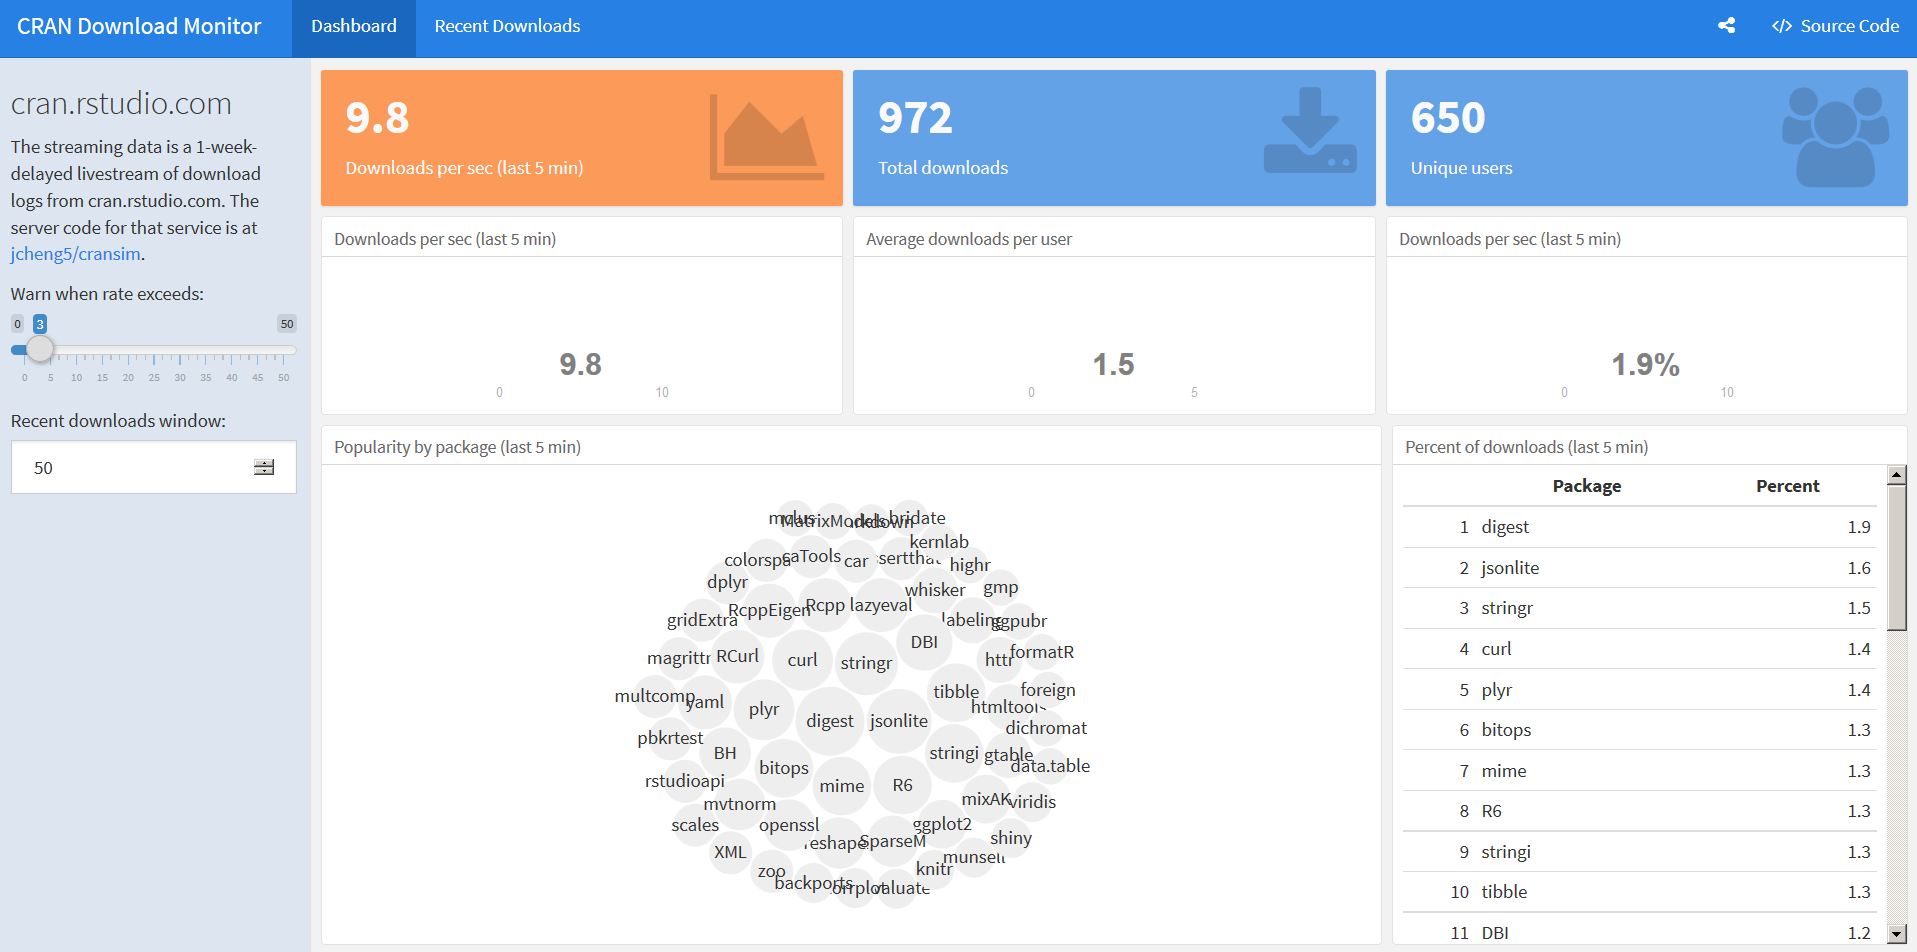
\includegraphics{D:/Daten/GitHub/IntroR/buildingblocks/figure/CRANdownloads.PNG}
\caption{Downloads vom CRAN Server}
\end{figure}

\end{frame}

\begin{frame}{Download R:}

\url{http://www.r-project.org/}

\begin{figure}
\centering
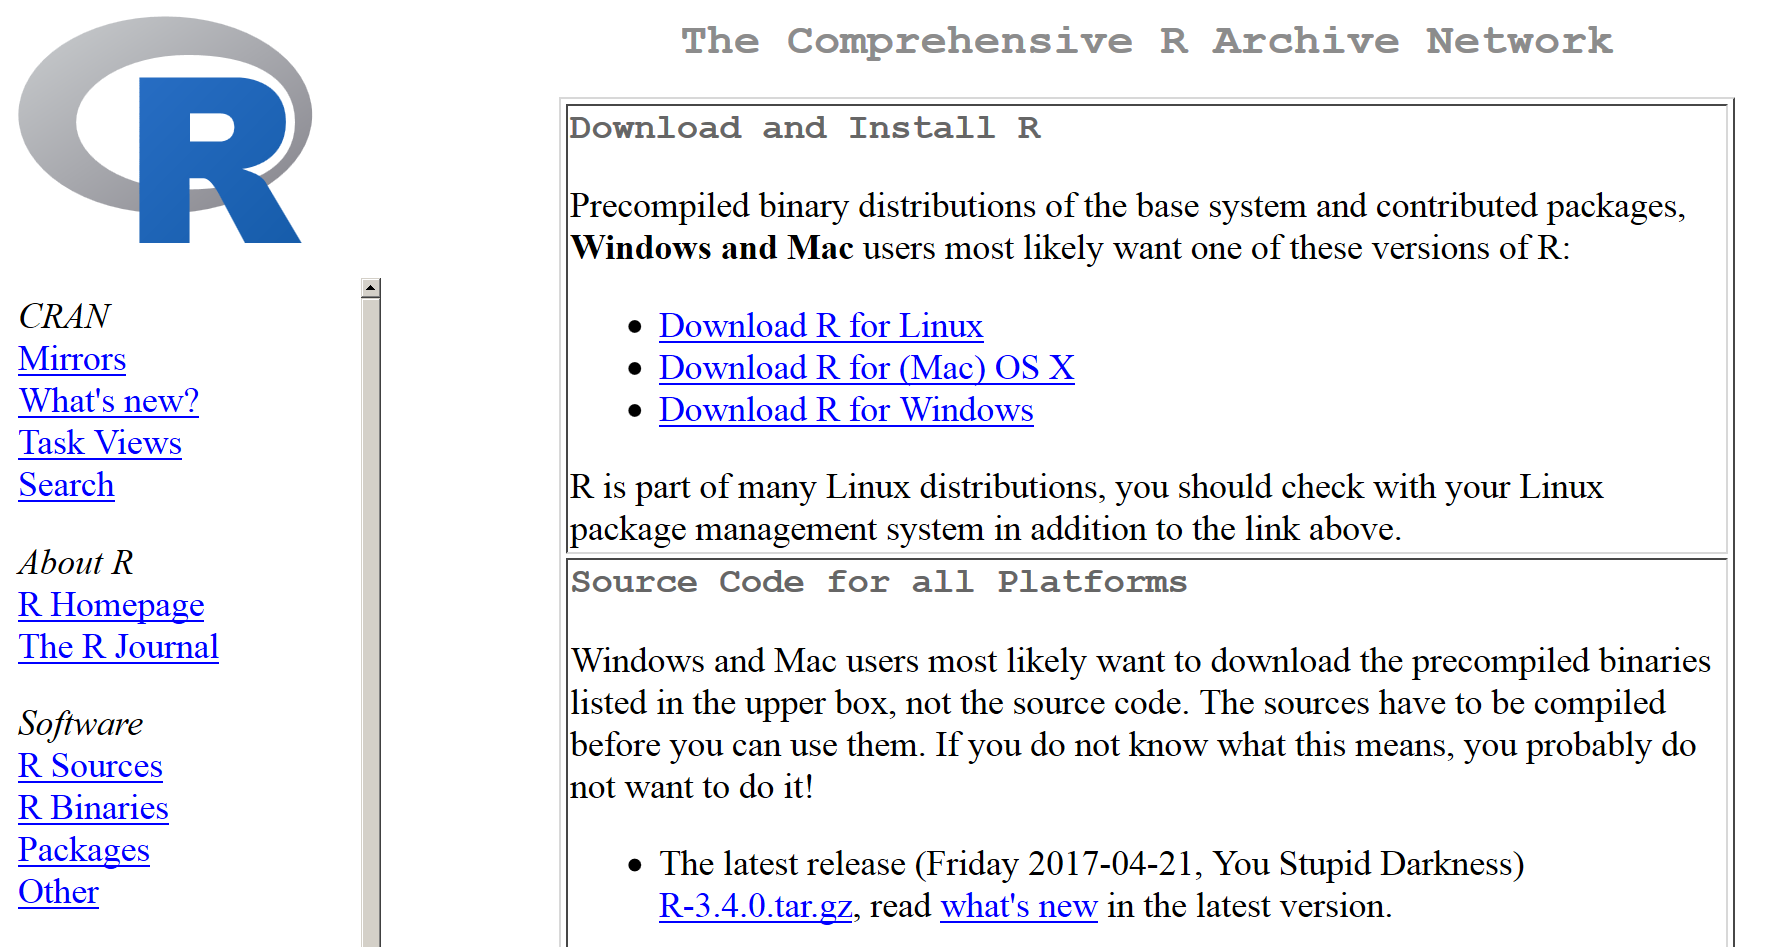
\includegraphics{D:/Daten/GitHub/IntroR/buildingblocks/figure/CRAN1picture.PNG}
\caption{The CRAN website}
\end{figure}

\end{frame}

\begin{frame}{Open Source Programm R}

\begin{block}{Das ist das Basis-R:}

\begin{figure}
\centering
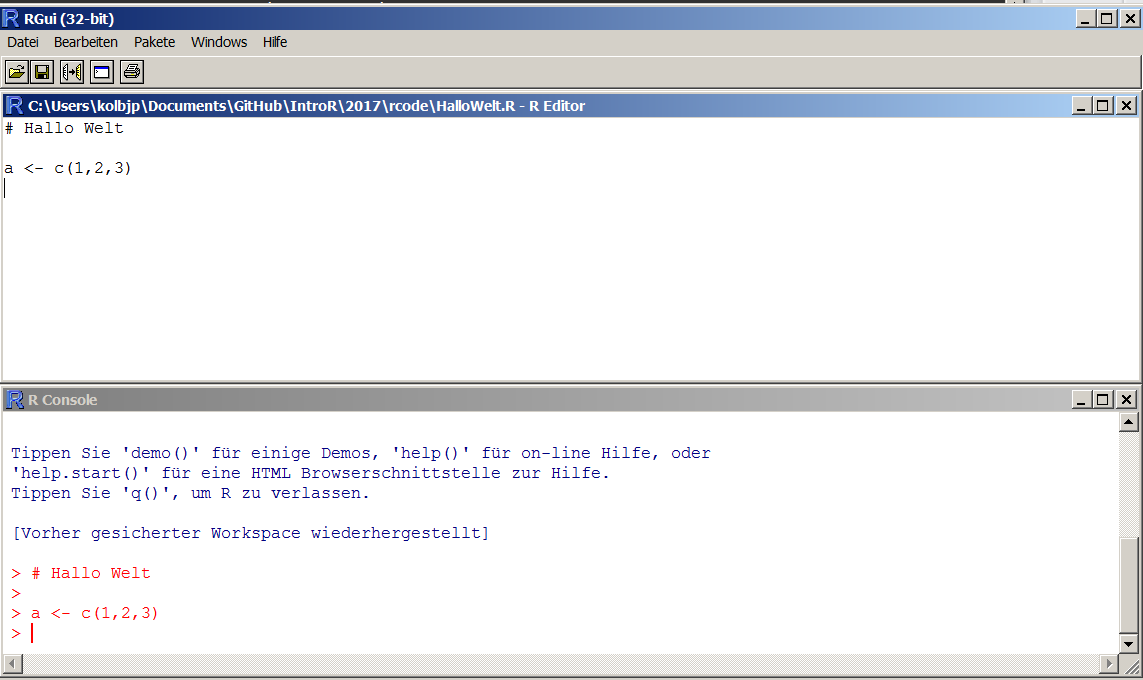
\includegraphics{D:/Daten/GitHub/IntroR/buildingblocks/figure/BasisR.PNG}
\caption{}
\end{figure}

\end{block}

\end{frame}

\begin{frame}{Graphical user interface}

Viele Leute nutzen ein
\href{https://en.wikipedia.org/wiki/Graphical_user_interface}{\textbf{Graphical
User Interface}} (GUI) oder ein
\href{https://en.wikipedia.org/wiki/Integrated_development_environment}{\textbf{Integrated
Development Interface}} (IDE).

Aus den folgenden Gründen:

\begin{itemize}
\tightlist
\item
  Syntax-Hervorhebung
\item
  Auto-Vervollständigung
\item
  Bessere Übersicht über Graphiken, Pakete, Dateien, \ldots{}
\end{itemize}

\end{frame}

\begin{frame}{RStudio}

\begin{figure}
\centering
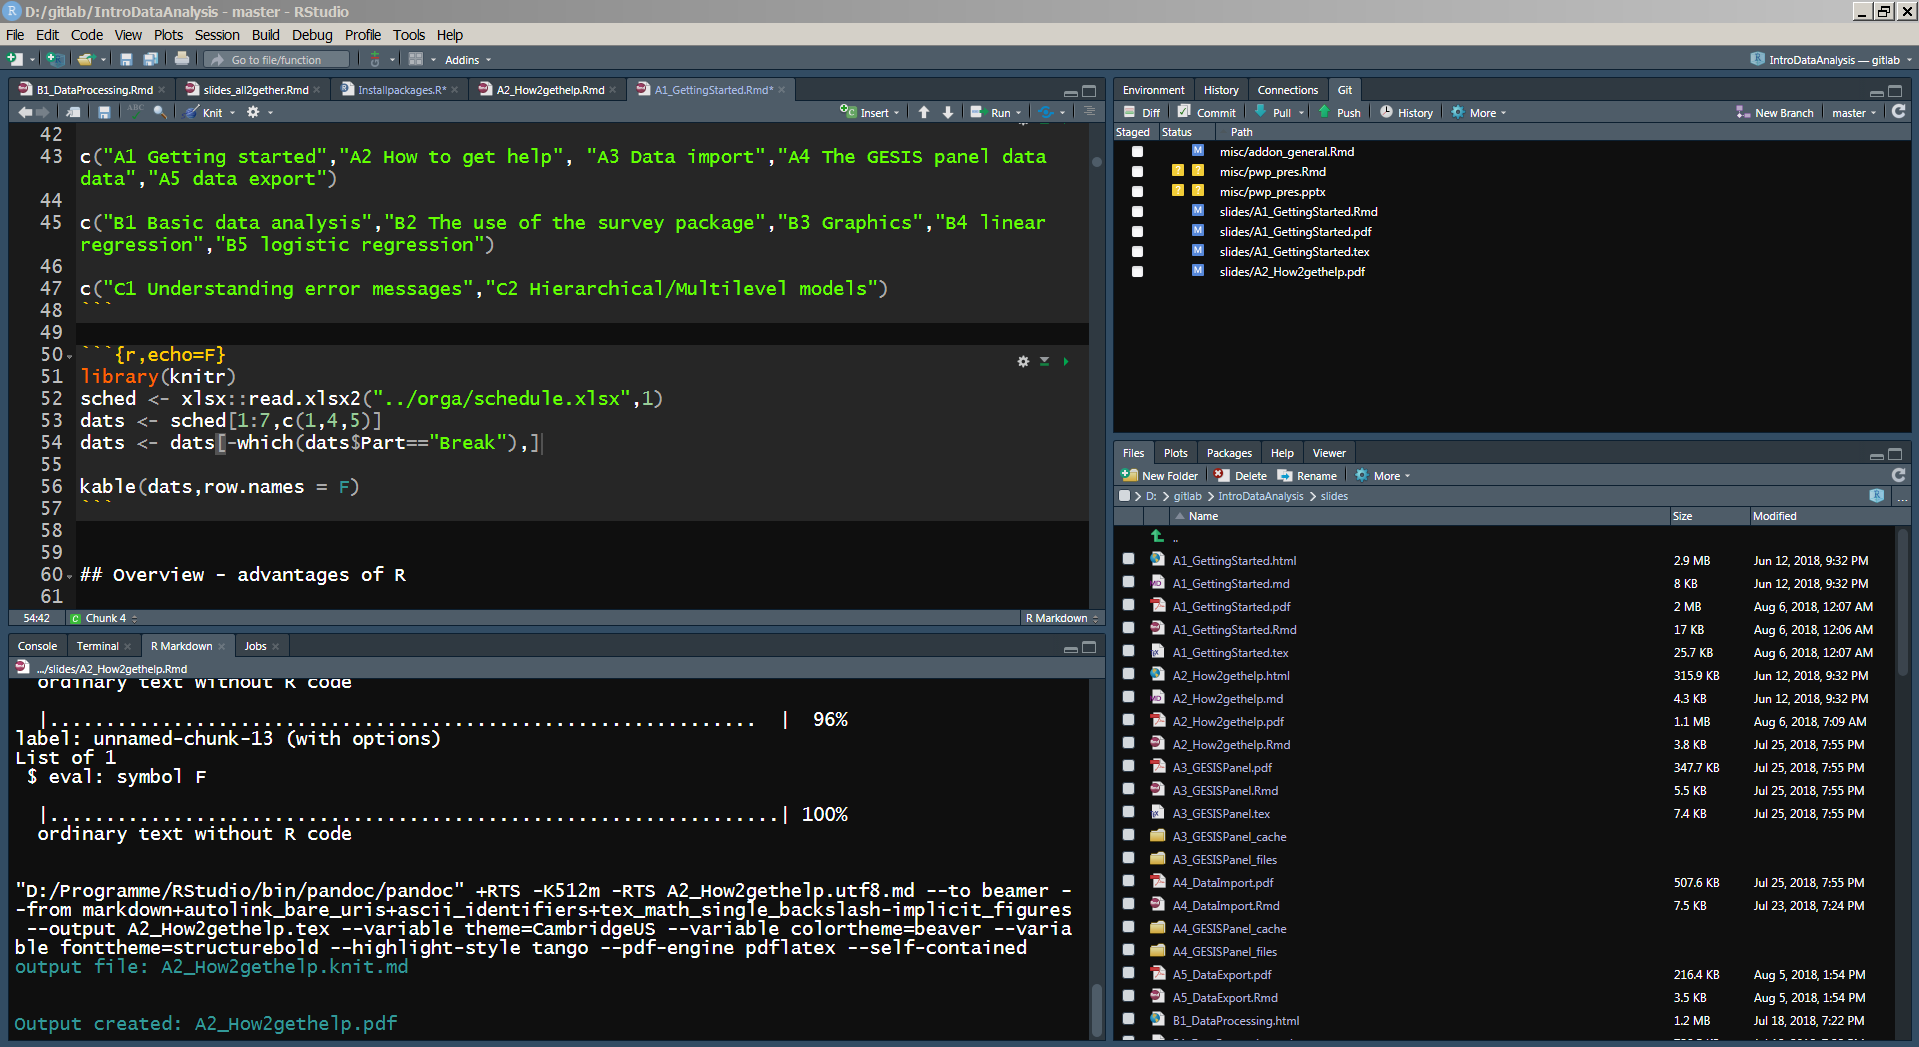
\includegraphics{D:/Daten/GitHub/IntroR/buildingblocks/figure/RstudioExample.PNG}
\caption{}
\end{figure}

\end{frame}

\begin{frame}[fragile]{Übung - Vorbereitung}

\begin{itemize}
\item
  Schaue, ob R auf dem Computer installiert ist
\item
  Wenn nicht, lade \href{r-project.org}{\textbf{R}} herunter und
  installiere es.
\item
  Prüfe ob Rstudio installiert ist.
\item
  Wenn nicht - \href{http://www.rstudio.com/}{\textbf{installiere}}
  Rstudio.
\item
  Starte RStudio. Gehe in die Konsole (meistens Fenster unten links) und
  tippe
\item
  Wenn noch kein Skript geöffnet im oberen linken Teil von Rstudio
  geöffnet ist, gehe zum Menü und öffne ein neues Skript. Checks das
  Datum mit \texttt{date()} und die R version mit
  \texttt{sessionInfo()}.
\end{itemize}

\end{frame}

\begin{frame}{Erste Schritte}

\end{frame}

\begin{frame}[fragile]{R ist eine objektorientierte Sprache.}

\begin{block}{Vektoren und Zuweisungen}

\begin{itemize}
\tightlist
\item
  \texttt{\textless{}-} ist der Zuweisungsoperator
\end{itemize}

\begin{Shaded}
\begin{Highlighting}[]
\NormalTok{b <-}\StringTok{ }\KeywordTok{c}\NormalTok{(}\DecValTok{1}\NormalTok{,}\DecValTok{2}\NormalTok{) }\CommentTok{# create an object with the numbers 1 and 2}
\end{Highlighting}
\end{Shaded}

\begin{itemize}
\tightlist
\item
  Auf dieses Objekt kann eine Funktion angewendet werden:
\end{itemize}

\begin{Shaded}
\begin{Highlighting}[]
\KeywordTok{mean}\NormalTok{(b) }\CommentTok{# computes the mean}
\end{Highlighting}
\end{Shaded}

\begin{verbatim}
## [1] 1.5
\end{verbatim}

Mit diesen Funktionen können wir etwas über die Eigenschaften des
Objekts erfahren:

\begin{Shaded}
\begin{Highlighting}[]
\KeywordTok{length}\NormalTok{(b) }\CommentTok{# b has the length 2}
\end{Highlighting}
\end{Shaded}

\begin{verbatim}
## [1] 2
\end{verbatim}

\end{block}

\begin{block}{Objektstruktur}

\begin{Shaded}
\begin{Highlighting}[]
\KeywordTok{str}\NormalTok{(b) }\CommentTok{# b is a numeric vector}
\end{Highlighting}
\end{Shaded}

\begin{verbatim}
##  num [1:2] 1 2
\end{verbatim}

\end{block}

\end{frame}

\begin{frame}[fragile]{Übung - Zuweisungen und Funktionen}

Erstellen Sie einen Vektor \texttt{b} mit den Zahlen von 1 bis 5 und
berechnen Sie\ldots{}.

\begin{enumerate}
\def\labelenumi{\arabic{enumi}.}
\item
  den Mittelwert
\item
  die Varianz
\item
  die Standardabweichung
\item
  die Quadratwurzel aus dem Mittelwert
\end{enumerate}

\end{frame}

\begin{frame}[fragile]{Wie bekomme ich Hilfe?}

\begin{itemize}
\tightlist
\item
  \href{http://itfeature.com/tag/how-to-get-help-in-r}{\textbf{Um Hilfe
  im Allgemeinen zu bekommen:}}
\end{itemize}

\begin{Shaded}
\begin{Highlighting}[]
\KeywordTok{help.start}\NormalTok{()}
\end{Highlighting}
\end{Shaded}

\begin{itemize}
\tightlist
\item
  \href{https://www.r-project.org/help.html}{\textbf{Online-Dokumentation
  für die meisten Funktionen:}}
\end{itemize}

\begin{Shaded}
\begin{Highlighting}[]
\KeywordTok{help}\NormalTok{(name)}
\end{Highlighting}
\end{Shaded}

\begin{itemize}
\tightlist
\item
  Benutze \texttt{?}, um Hilfe zu bekommen
\end{itemize}

\begin{Shaded}
\begin{Highlighting}[]
\NormalTok{?mean}
\end{Highlighting}
\end{Shaded}

\begin{itemize}
\tightlist
\item
  \texttt{example(lm)} liefert ein Beispiel für die lineare Regression
\end{itemize}

\begin{Shaded}
\begin{Highlighting}[]
\KeywordTok{example}\NormalTok{(lm)}
\end{Highlighting}
\end{Shaded}

\end{frame}

\begin{frame}[fragile]{Vignetten}

\begin{itemize}
\tightlist
\item
  Eine Vignette ist ein Papier, das die wichtigsten Funktionen eines
  Pakets darstellt.
\item
  Sie enthalten viele reproduzierbare Beispiele.
\item
  Vignetten sind ein neues Werkzeug, deshalb hat nicht jedes Paket eine
  Vignette.
\end{itemize}

\begin{Shaded}
\begin{Highlighting}[]
\KeywordTok{browseVignettes}\NormalTok{()}
\end{Highlighting}
\end{Shaded}

\begin{itemize}
\tightlist
\item
  Um eine Vignette zu bekommen:
\end{itemize}

\begin{Shaded}
\begin{Highlighting}[]
\KeywordTok{vignette}\NormalTok{(}\StringTok{"osmdata"}\NormalTok{)}
\end{Highlighting}
\end{Shaded}

\end{frame}

\begin{frame}{Ein Beispiel für eine Vignette - Das Paket
\texttt{osmdata}}

\begin{figure}
\centering
\includegraphics{D:/Daten/GitHub/IntroR/buildingblocks/figure/ex_osmdata_vignette.PNG}
\caption{}
\end{figure}

\end{frame}

\begin{frame}[fragile]{\href{http://r-pkgs.had.co.nz/demo.html}{\textbf{Demos}}}

\begin{itemize}
\tightlist
\item
  für manche Pakete gibt es Demos:
\end{itemize}

\begin{Shaded}
\begin{Highlighting}[]
\KeywordTok{demo}\NormalTok{() }\CommentTok{# zeigt alle verfügbaren Demos}
\KeywordTok{demo}\NormalTok{(}\DataTypeTok{package =} \StringTok{"httr"}\NormalTok{) }\CommentTok{# Zeigt alle Demos in einem Paket}

\CommentTok{# Ein spezifisches Demo laufen lassen:}
\KeywordTok{demo}\NormalTok{(}\StringTok{"oauth1-twitter"}\NormalTok{, }\DataTypeTok{package =} \StringTok{"httr"}\NormalTok{) }
\end{Highlighting}
\end{Shaded}

\begin{itemize}
\tightlist
\item
  Wenn ein Demo gestartet wird, ist der zugehörige Code in der Konsole
  sichtbar
\end{itemize}

\begin{Shaded}
\begin{Highlighting}[]
\KeywordTok{demo}\NormalTok{(nlm)}
\end{Highlighting}
\end{Shaded}

\begin{figure}
\centering
\includegraphics{D:/Daten/GitHub/IntroR/buildingblocks/figure/demonlm.PNG}
\caption{}
\end{figure}

\end{frame}

\begin{frame}[fragile]{Die Funktion \texttt{apropos}}

\begin{itemize}
\tightlist
\item
  durchsucht alles über den angegebenen String:
\end{itemize}

\begin{Shaded}
\begin{Highlighting}[]
\KeywordTok{apropos}\NormalTok{(}\StringTok{"lm"}\NormalTok{)}
\end{Highlighting}
\end{Shaded}

\begin{verbatim}
##  [1] ".colMeans"       ".lm.fit"         "colMeans"       
##  [4] "confint.lm"      "contr.helmert"   "dummy.coef.lm"  
##  [7] "getAllMethods"   "glm"             "glm.control"    
## [10] "glm.fit"         "KalmanForecast"  "KalmanLike"     
## [13] "KalmanRun"       "KalmanSmooth"    "kappa.lm"       
## [16] "lm"              "lm.fit"          "lm.influence"   
## [19] "lm.wfit"         "model.matrix.lm" "nlm"            
## [22] "nlminb"          "predict.glm"     "predict.lm"     
## [25] "residuals.glm"   "residuals.lm"    "summary.glm"    
## [28] "summary.lm"
\end{verbatim}

\begin{itemize}
\tightlist
\item
  Funktion kann auch mit
  \href{https://de.wikipedia.org/wiki/Regul\%C3\%A4rer_Ausdruck}{\textbf{regulären
  Ausdrücken}} verwendet werden\ldots{}
\end{itemize}

\begin{Shaded}
\begin{Highlighting}[]
\NormalTok{?}\StringTok{"regular expression"}
\end{Highlighting}
\end{Shaded}

\begin{Shaded}
\begin{Highlighting}[]
\KeywordTok{help.search}\NormalTok{(}\StringTok{"^glm"}\NormalTok{)}
\end{Highlighting}
\end{Shaded}

\begin{itemize}
\tightlist
\item
  \texttt{??} ist ein Synonym für \texttt{help.search}
\end{itemize}

\end{frame}

\begin{frame}[fragile]{\href{http://search.r-project.org/cgi-bin/namazu.cgi?query=glm\&max=20\&result=normal\&sort=score\&idxname=functions\&idxname=vignettes\&idxname=views}{\textbf{Suchmaschine
für die R-Seite}}}

\begin{Shaded}
\begin{Highlighting}[]
\KeywordTok{RSiteSearch}\NormalTok{(}\StringTok{"glm"}\NormalTok{)}
\end{Highlighting}
\end{Shaded}

\begin{figure}
\centering
\includegraphics{D:/Daten/GitHub/IntroR/buildingblocks/figure/rsitesearch.PNG}
\caption{}
\end{figure}

\end{frame}

\begin{frame}[fragile]{Nutzung von Suchmaschinen}

\begin{itemize}
\tightlist
\item
  Ich nutze \href{}{\textbf{duckduckgo.de:}}
\end{itemize}

\begin{verbatim}
R-project + "was ich schon immer wissen wollte" 
\end{verbatim}

\begin{itemize}
\tightlist
\item
  das funktioniert natürlich für alle Suchmaschinen!
\end{itemize}

\begin{figure}
\centering
\includegraphics{D:/Daten/GitHub/IntroR/buildingblocks/figure/duckduckgo.PNG}
\caption{}
\end{figure}

\end{frame}

\begin{frame}{\href{http://stackoverflow.com/}{\textbf{Stackoverflow}}}

\begin{itemize}
\tightlist
\item
  Für alle Fragen zum programmieren
\item
  Ist nicht auf R fokussiert - aber es gibt
  \href{https://stackoverflow.com/tags/r/info}{\textbf{viele
  Diskussionen zu R-Fragen}}
\item
  Sehr detailierte Diskussionen
\end{itemize}

\begin{figure}
\centering
\includegraphics{D:/Daten/GitHub/IntroR/buildingblocks/figure/StackoverflowEx.PNG}
\caption{Stackoverflow Beispiel}
\end{figure}

\end{frame}

\begin{frame}{Ein Schummelzettel für Basis R}

\url{https://www.rstudio.com/resources/cheatsheets/}

\begin{figure}
\centering
\includegraphics{D:/Daten/GitHub/IntroR/buildingblocks/figure/basercheatsheet.PNG}
\caption{\textbf{Cheatsheet BaseR}}
\end{figure}

\end{frame}

\begin{frame}{Mehr Schummelzettel}

\begin{figure}
\centering
\includegraphics{D:/Daten/GitHub/IntroR/buildingblocks/figure/cheatsheets.PNG}
\caption{}
\end{figure}

\end{frame}

\begin{frame}{\href{http://www.statmethods.net/interface/help.html}{\textbf{Quick
R}}}

\begin{itemize}
\tightlist
\item
  Immer mit vielen Beispielen und Hilfen bezüglich eines Themas
\item
  Beispiel:
  \href{http://www.statmethods.net/interface/help.html}{\textbf{Quick R
  - Getting Help}}
\end{itemize}

\begin{figure}
\centering
\includegraphics{D:/Daten/GitHub/IntroR/buildingblocks/figure/quickR.PNG}
\caption{}
\end{figure}

\end{frame}

\begin{frame}{Weitere Links}

\begin{itemize}
\tightlist
\item
  \href{https://www.r-project.org/help.html}{\textbf{Überblick - wie
  bekommt man Hilfe in R}}
\end{itemize}

\begin{figure}
\centering
\includegraphics{D:/Daten/GitHub/IntroR/buildingblocks/figure/gettingHelp.PNG}
\caption{}
\end{figure}

\begin{itemize}
\item
  \href{http://rprogramming.net/}{\textbf{Eine Liste mit HowTo`s}}
\item
  \href{https://www.personality-project.org/r/r.commands.html}{\textbf{Eine
  Liste mit den wichtigsten R-Befehlen}}
\end{itemize}

\end{frame}

\begin{frame}[fragile]{Aufgabe A2A
\href{http://web.math.ku.dk/~helle/R-intro/exercises.pdf}{\textbf{Hilfe
bekommen}}}

\begin{block}{LABORATORY FOR APPLIED STATISTICS: Intro to R -
\href{http://web.math.ku.dk/~helle/R-intro/exercises.pdf}{\textbf{Exercises}}
für diese Aufgabe}

\begin{itemize}
\item
  Versuchen Sie den Befehl \texttt{?which.min}. Dies öffnet eine
  Hilfeseite im unteren rechten Fenster von RStudio. Was macht die
  Funktion?
\item
  Sie müssen den Namen der Funktion kennen, um die Hilfeseite wie oben
  beschrieben zu öffnen. Manchmal (oft, sogar) kennen Sie den Namen der
  R-Funktionen nicht; dann kann Ihnen eine
  \href{https://duckduckgo.com/}{\textbf{Suchmaschine}} helfen.
  Versuchen Sie zum Beispiel, den Text \texttt{R\ minimum\ vector} zu
  suchen.
\end{itemize}

\end{block}

\end{frame}

\begin{frame}{\href{https://stats.idre.ucla.edu/r/seminars/intro/}{\textbf{Wo
man Routinen findet}}}

\begin{itemize}
\tightlist
\item
  Viele Funktionen sind in Basis-R enthalten.
\item
  Viele spezifische Funktionen sind in zusätzliche Bibliotheken
  integriert.
\item
  R kann modular durch sogenannte Pakete oder Bibliotheken erweitert
  werden.
\item
  Die wichtigsten Pakete, die auf CRAN gehostet werden (13610 at Di Jan
  08)
\item
  Weitere Pakete findet man z.B. unter
  \href{www.bioconductor.org}{\textbf{bioconductor}}
\end{itemize}

\end{frame}

\begin{frame}{\href{https://www.youtube.com/watch?v=kKI9--Opmso}{Übersicht
R-Pakete}}

\begin{figure}
\centering
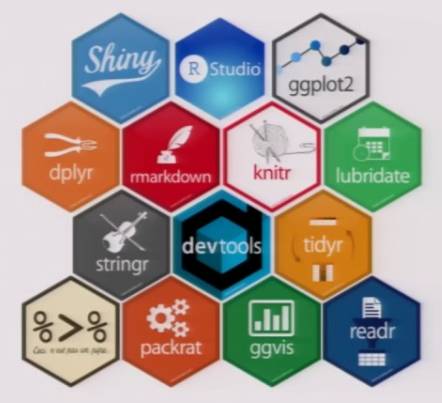
\includegraphics{figure/packages_overview.PNG}
\caption{Overview R-packages}
\end{figure}

\end{frame}

\begin{frame}[fragile]{Installation von Paketen}

\begin{itemize}
\tightlist
\item
  Die Anführungszeichen um den Paketnamen herum sind für den Befehl
  \texttt{install.packages} notwendig.
\item
  Sie sind optional für den Befehl \texttt{library}.
\item
  Man kann auch \texttt{require} anstelle von \texttt{library}
  verwenden.
\end{itemize}

\begin{Shaded}
\begin{Highlighting}[]
\KeywordTok{install.packages}\NormalTok{(}\StringTok{"raster"}\NormalTok{)}

\KeywordTok{library}\NormalTok{(raster)}
\end{Highlighting}
\end{Shaded}

\end{frame}

\begin{frame}{Installation von Paketen mit RStudio}

\begin{figure}
\centering
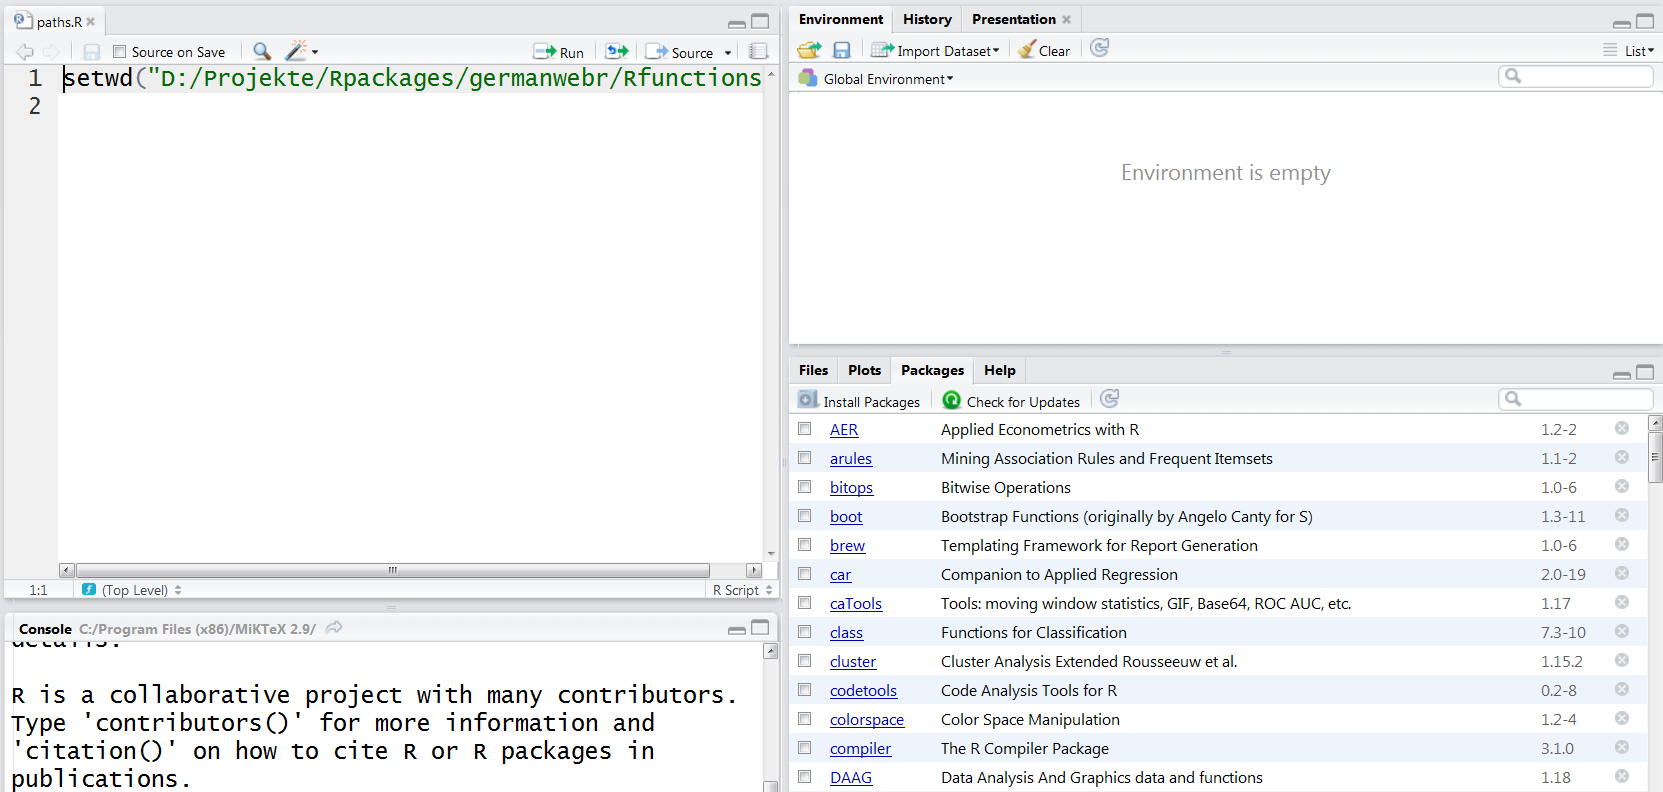
\includegraphics{figure/PaketeRstudio.PNG}
\caption{Package installation with Rstudio}
\end{figure}

\end{frame}

\begin{frame}{Bestehende Pakete und Installation}

\begin{figure}
\centering
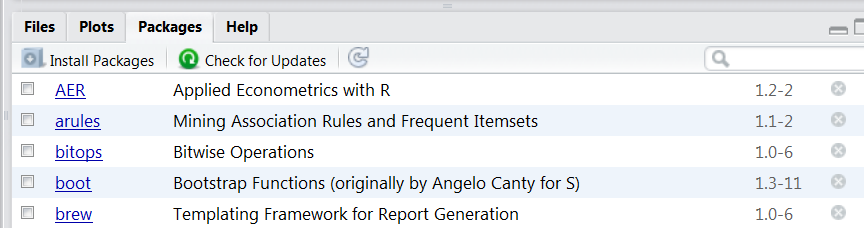
\includegraphics{figure/packages3.PNG}
\caption{Existing packages}
\end{figure}

\end{frame}

\begin{frame}[fragile]{Übersicht über viele nützliche Pakete:}

\begin{itemize}
\tightlist
\item
  Luhmann -
  \href{http://www.beltz.de/fileadmin/beltz/downloads/OnlinematerialienPVU/28090_Luhmann/Verwendete\%20Pakete.pdf}{\textbf{Übersicht
  mit vielen nützlichen Paketen}}
\end{itemize}

\begin{block}{Weitere interessante Pakete:}

\begin{itemize}
\tightlist
\item
  Mit dem Paket \texttt{leaflet} kann man interaktive Karten erstellen.
\item
  Das Paket \texttt{tmap} zur Erstellung von thematischen Karten.
\item
  \href{http://www.r-bloggers.com/tag/maptools/}{\textbf{Paket
  \texttt{maptools} um Karten zu erzeugen}}
\item
  Das Paket \texttt{sf} - bietet Zugang zu
  \href{https://de.wikipedia.org/wiki/Simple_Feature_Access}{\textbf{simple
  features}}.
\end{itemize}

\begin{figure}
\centering

\includegraphics{figure/logo_sf.PNG}
\caption{}
\end{figure}

\end{block}

\end{frame}

\begin{frame}[fragile]{Pakete aus verschiedenen Quellen installieren}

\begin{block}{Pakete vom CRAN Server installieren}

\begin{Shaded}
\begin{Highlighting}[]
\KeywordTok{install.packages}\NormalTok{(}\StringTok{"lme4"}\NormalTok{)}
\end{Highlighting}
\end{Shaded}

\end{block}

\begin{block}{Pakete vom Bioconductor Server installieren}

\begin{Shaded}
\begin{Highlighting}[]
\KeywordTok{source}\NormalTok{(}\StringTok{"https://bioconductor.org/biocLite.R"}\NormalTok{)}
\KeywordTok{biocLite}\NormalTok{(}\KeywordTok{c}\NormalTok{(}\StringTok{"GenomicFeatures"}\NormalTok{, }\StringTok{"AnnotationDbi"}\NormalTok{))}
\end{Highlighting}
\end{Shaded}

\end{block}

\begin{block}{Pakete von Github installieren}

\begin{Shaded}
\begin{Highlighting}[]
\KeywordTok{install.packages}\NormalTok{(}\StringTok{"devtools"}\NormalTok{)}
\KeywordTok{library}\NormalTok{(devtools)}

\KeywordTok{install_github}\NormalTok{(}\StringTok{"hadley/maptools"}\NormalTok{)}
\end{Highlighting}
\end{Shaded}

\end{block}

\end{frame}

\begin{frame}{Wie bekomme ich einen Überblick?}

\begin{itemize}
\item
  Entdecke Pakete, die kürzlich auf den
  \href{https://mran.microsoft.com/packages/}{\textbf{CRAN}} Server
  hochgeladen wurden
\item
  Nutze eine Shiny Web-App, die
  \href{https://gallery.shinyapps.io/cran-gauge/}{\textbf{Pakete
  anzeigt, die kürzlich von CRAN}} heruntergeladen wurden.
\item
  Werfe einen Blick auf eine
  \href{https://support.rstudio.com/hc/en-us/articles/201057987-Quick-list-of-useful-R-packages}{\textbf{Quick-Liste
  nützlicher Pakete}}
\item
  \ldots{}., oder auf eine Liste mit den
  \href{http://www.computerworld.com/article/2921176/business-intelligence/great-r-packages-for-data-import-wrangling-visualization.html}{\textbf{besten
  Paketen für die Datenverarbeitung und -analyse}},\ldots{}..
\item
  \ldots{}., oder schaue unter
  \href{https://www.r-bloggers.com/the-50-most-used-r-packages/}{\textbf{die
  50 meistgenutzten Pakete}}
\end{itemize}

\end{frame}

\begin{frame}[fragile]{CRAN Task Views}

\begin{itemize}
\tightlist
\item
  Bezüglich mancher Themen gibt es einen Überblick über alle wichtigen
  Pakete - (\href{https://cran.r-project.org/web/views/}{\textbf{CRAN
  Task Views}})
\item
  Momentan gibt es 35 Task Views.
\item
  Alle Pakete einer Task-View können mit folgendem Befehl installiert
  werden:
  \href{https://mran.microsoft.com/rpackages/}{\textbf{command:}}
\end{itemize}

\begin{Shaded}
\begin{Highlighting}[]
\KeywordTok{install.packages}\NormalTok{(}\StringTok{"ctv"}\NormalTok{)}
\KeywordTok{library}\NormalTok{(}\StringTok{"ctv"}\NormalTok{)}
\KeywordTok{install.views}\NormalTok{(}\StringTok{"Spatial"}\NormalTok{)}
\end{Highlighting}
\end{Shaded}

\begin{figure}
\centering
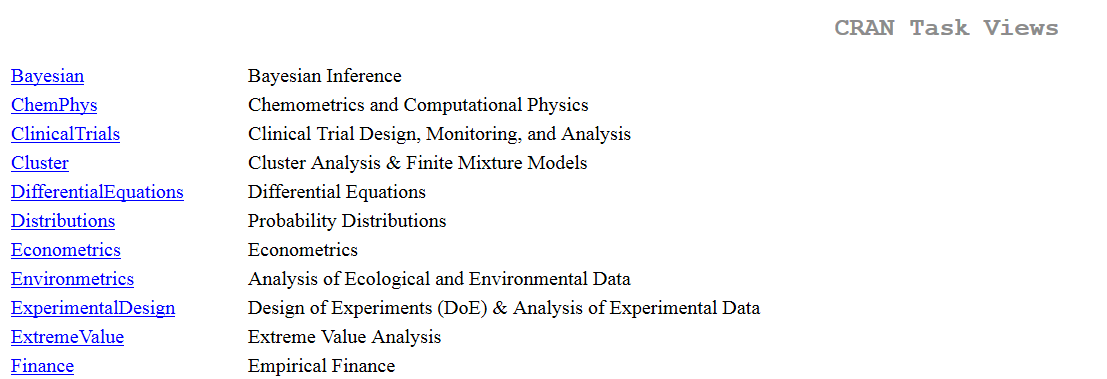
\includegraphics{figure/CRANtaskViews.PNG}
\caption{}
\end{figure}

\end{frame}

\begin{frame}{Übung - zusätzliche Pakete}

Geh bspw. auf \url{https://cran.r-project.org/} und suche nach
Paketen\ldots{}

\begin{itemize}
\tightlist
\item
  die sich für interaktive Karten eignen.
\item
  mit denen man thematische Karten erstellen kann
\item
  mit denen man die räumliche Distanz berechnen kann
\item
  mit denen man eine Satelitenkarte bekommen kann
\end{itemize}

\end{frame}

\begin{frame}[fragile]{Beispiel zu Campingplätzen}

\begin{itemize}
\tightlist
\item
  Die Daten stammen von:
\end{itemize}

\url{http://www.openstreetmap.de/}

\begin{itemize}
\tightlist
\item
  Dabei wird die Overpass API genutzt:
\end{itemize}

\url{http://wiki.openstreetmap.org/wiki/Overpass_API}

\begin{Shaded}
\begin{Highlighting}[]
\NormalTok{url <-}\StringTok{ "https://raw.githubusercontent.com/Japhilko/}
\StringTok{GeoData/master/2015/data/CampSites_Germany.csv"}
\end{Highlighting}
\end{Shaded}

\begin{Shaded}
\begin{Highlighting}[]
\NormalTok{CampSites <-}\StringTok{ }\KeywordTok{read.csv}\NormalTok{(url)}
\end{Highlighting}
\end{Shaded}

\end{frame}

\begin{frame}{Überblick über Daten zu Campingplätzen}

\begin{longtable}[]{@{}rlll@{}}
\toprule
X & name & tourism & website\tabularnewline
\midrule
\endhead
1 & Campingplatz Winkelbachtal & camp\_site &
\url{http://www.gruibingen.de/campingplatz.html}\tabularnewline
2 & Radler-Zeltplatz & camp\_site & NA\tabularnewline
3 & Campingplatz des Naturfreundehauses & camp\_site & NA\tabularnewline
4 & Campingplatz Am Aichstruter Stausee & camp\_site & NA\tabularnewline
5 & NA & camp\_site & NA\tabularnewline
6 & Kandern & camp\_site & NA\tabularnewline
7 & Campingplatz Baiersbronn-Obertal & camp\_site & NA\tabularnewline
8 & Campingplatz Schwabenmühle & camp\_site & NA\tabularnewline
\bottomrule
\end{longtable}

\end{frame}

\begin{frame}[fragile]{Notwendige Pakete}

\begin{block}{\href{https://cran.r-project.org/web/packages/magrittr/index.html}{\textbf{magrittr}}
- für den Pipe Operator in R:}

\begin{Shaded}
\begin{Highlighting}[]
\KeywordTok{library}\NormalTok{(}\StringTok{"magrittr"}\NormalTok{)}
\end{Highlighting}
\end{Shaded}

\href{https://rstudio.github.io/leaflet/}{leaflet} - um interaktive
Karten mit der JavaScript Bibliothek `Leaflet' zu erzeugen

\begin{Shaded}
\begin{Highlighting}[]
\KeywordTok{library}\NormalTok{(}\StringTok{"leaflet"}\NormalTok{)}
\end{Highlighting}
\end{Shaded}

\end{block}

\end{frame}

\begin{frame}[fragile]{Eine erste interaktive Karte}

\begin{Shaded}
\begin{Highlighting}[]
\KeywordTok{leaflet}\NormalTok{()}\OperatorTok
\StringTok{  }\KeywordTok{addTiles}\NormalTok{()}
\end{Highlighting}
\end{Shaded}

\begin{figure}
\centering
\includegraphics{D:/Daten/GitHub/IntroR/buildingblocks/figure/FirstLeaflet.PNG}
\caption{Hallo Leaflet}
\end{figure}

\end{frame}

\begin{frame}[fragile]{Auf eine Stadt zoomen}

\begin{Shaded}
\begin{Highlighting}[]
\KeywordTok{leaflet}\NormalTok{() }\OperatorTok
\StringTok{  }\KeywordTok{addTiles}\NormalTok{() }\OperatorTok
\StringTok{  }\KeywordTok{addMarkers}\NormalTok{(}\DataTypeTok{lng=}\FloatTok{8.456597}\NormalTok{, }\DataTypeTok{lat=}\FloatTok{49.48738}\NormalTok{,}
             \DataTypeTok{popup=}\StringTok{"Wo wir sind"}\NormalTok{)}
\end{Highlighting}
\end{Shaded}

\begin{figure}
\centering
\includegraphics{D:/Daten/GitHub/IntroR/buildingblocks/figure/leafletMZESMA.PNG}
\caption{}
\end{figure}

\end{frame}

\begin{frame}[fragile]{Eine interaktive Karte}

\begin{Shaded}
\begin{Highlighting}[]
\NormalTok{m <-}\StringTok{ }\KeywordTok{leaflet}\NormalTok{() }\OperatorTok
\StringTok{  }\KeywordTok{addTiles}\NormalTok{() }\OperatorTok\StringTok{  }
\StringTok{  }\KeywordTok{addMarkers}\NormalTok{(}\DataTypeTok{lng=}\NormalTok{CampSites}\OperatorTok{$}\NormalTok{lon, }
             \DataTypeTok{lat=}\NormalTok{CampSites}\OperatorTok{$}\NormalTok{lat, }
             \DataTypeTok{popup=}\NormalTok{CampSites}\OperatorTok{$}\NormalTok{name)}
\NormalTok{m}
\end{Highlighting}
\end{Shaded}

\end{frame}

\begin{frame}[fragile]{Das Paket \texttt{leaflet} - Visualisierung von
Geokodierung}

\begin{Shaded}
\begin{Highlighting}[]
\KeywordTok{library}\NormalTok{(}\StringTok{"tmaptools"}\NormalTok{)}
\NormalTok{gc_tma <-}\StringTok{ }\KeywordTok{geocode_OSM}\NormalTok{(}\StringTok{"Mannheim, GESIS"}\NormalTok{)}
\end{Highlighting}
\end{Shaded}

\begin{Shaded}
\begin{Highlighting}[]
\KeywordTok{library}\NormalTok{(leaflet)}
\KeywordTok{library}\NormalTok{(magrittr)}
\NormalTok{m <-}\StringTok{ }\KeywordTok{leaflet}\NormalTok{() }\OperatorTok
\KeywordTok{addTiles}\NormalTok{() }\OperatorTok
\KeywordTok{addMarkers}\NormalTok{(}\DataTypeTok{lng=}\FloatTok{8.463061}\NormalTok{ , }\DataTypeTok{lat=}\FloatTok{49.485736}\NormalTok{ , }
           \DataTypeTok{popup=}\StringTok{"GESIS Mannheim"}\NormalTok{)}
\NormalTok{m}
\end{Highlighting}
\end{Shaded}

\end{frame}

\begin{frame}[fragile]{\href{https://rstudio.github.io/leaflet/basemaps.html}{Stamen
als Hintergrundkarte}}

\begin{Shaded}
\begin{Highlighting}[]
\NormalTok{m }\OperatorTok\StringTok{ }\KeywordTok{addProviderTiles}\NormalTok{(}\StringTok{"Stamen.Toner"}\NormalTok{)}
\end{Highlighting}
\end{Shaded}

\begin{figure}
\centering
\includegraphics{D:/Daten/GitHub/IntroR/buildingblocks/figure/InteractiveStamen.PNG}
\caption{Eine Stamen Karte als Hintergrund}
\end{figure}

\end{frame}

\begin{frame}[fragile]{CartoDB als Hintergrund}

\begin{Shaded}
\begin{Highlighting}[]
\NormalTok{m }\OperatorTok\StringTok{ }\KeywordTok{addProviderTiles}\NormalTok{(}\StringTok{"CartoDB.Positron"}\NormalTok{)}
\end{Highlighting}
\end{Shaded}

\begin{figure}
\centering
\includegraphics{D:/Daten/GitHub/IntroR/buildingblocks/figure/CartoDBInteractive.PNG}
\caption{CartoDB als Hintergrund}
\end{figure}

\begin{itemize}
\item
  \href{https://carto.com/attribution}{CartoDB}
\item
  \href{https://www.mapbox.com/help/how-web-maps-work/}{Info zu Map
  Tiles}
\end{itemize}

\end{frame}

\begin{frame}[fragile]{\href{http://leaflet-extras.github.io/leaflet-providers/preview/index.html}{Mehr
Hintergründe}}

\begin{Shaded}
\begin{Highlighting}[]
\NormalTok{m }\OperatorTok\StringTok{ }\KeywordTok{addProviderTiles}\NormalTok{(}\StringTok{"NASAGIBS.ViirsEarthAtNight2012"}\NormalTok{)}
\end{Highlighting}
\end{Shaded}

\begin{figure}
\centering
\includegraphics{D:/Daten/GitHub/IntroR/buildingblocks/figure/LightsInteractive.PNG}
\caption{Lichter der Nacht}
\end{figure}

\end{frame}

\begin{frame}[fragile]{Mehr Informationen hinzufügen}

\begin{Shaded}
\begin{Highlighting}[]
\NormalTok{popupInfo <-}\StringTok{ }\KeywordTok{paste}\NormalTok{(CampSites}\OperatorTok{$}\NormalTok{name,}\StringTok{"}\CharTok{\textbackslash{}n}\StringTok{"}\NormalTok{,CampSites}\OperatorTok{$}\NormalTok{website)}
\end{Highlighting}
\end{Shaded}

\begin{Shaded}
\begin{Highlighting}[]
\NormalTok{m <-}\StringTok{ }\KeywordTok{leaflet}\NormalTok{() }\OperatorTok
\StringTok{  }\KeywordTok{addTiles}\NormalTok{() }\OperatorTok\StringTok{  }\CommentTok{# Add default OpenStreetMap map tiles}
\StringTok{  }\KeywordTok{addMarkers}\NormalTok{(}\DataTypeTok{lng=}\NormalTok{CampSites}\OperatorTok{$}\NormalTok{lon, }
             \DataTypeTok{lat=}\NormalTok{CampSites}\OperatorTok{$}\NormalTok{lat, }
             \DataTypeTok{popup=}\NormalTok{popupInfo)}
\NormalTok{m}
\end{Highlighting}
\end{Shaded}

Das Ergebnis ist hier:

\url{http://rpubs.com/Japhilko82/CampSitesHL}

\end{frame}

\begin{frame}{Die resultierende Karte}

\begin{figure}
\centering
\includegraphics{D:/Daten/GitHub/IntroR/buildingblocks/figure/Germany_Campsites.PNG}
\caption{Campingplätze in Deutschland}
\end{figure}

\end{frame}

\begin{frame}{Popups in einer interactiven Karte}

\begin{figure}
\centering
\includegraphics{D:/Daten/GitHub/IntroR/buildingblocks/figure/Camping_Mannheim.PNG}
\caption{Camping Mannheim}
\end{figure}

Ich hab die Ergebnisse hochgeladen:

\url{http://rpubs.com/Japhilko82/Campsites}

\end{frame}

\begin{frame}{Wie man auf Rpubs publizieren kann}

\begin{figure}
\centering
\includegraphics{D:/Daten/GitHub/IntroR/buildingblocks/figure/PublishCampSitesGermany.PNG}
\caption{Publizieren auf Rpubs}
\end{figure}

\end{frame}

\begin{frame}[fragile]{Ein weiteres Beispiel - Weltkulturerbe}

\begin{Shaded}
\begin{Highlighting}[]
\NormalTok{url <-}\StringTok{ "https://raw.githubusercontent.com/Japhilko/}
\StringTok{GeoData/master/2015/data/whcSites.csv"}

\NormalTok{whcSites <-}\StringTok{ }\KeywordTok{read.csv}\NormalTok{(url) }
\end{Highlighting}
\end{Shaded}

\end{frame}

\begin{frame}[fragile]{Eine interaktive Karte erstellen}

\begin{Shaded}
\begin{Highlighting}[]
\NormalTok{m <-}\StringTok{ }\KeywordTok{leaflet}\NormalTok{() }\OperatorTok
\StringTok{  }\KeywordTok{addTiles}\NormalTok{() }\OperatorTok\StringTok{  }\CommentTok{# Add default OpenStreetMap map tiles}
\StringTok{  }\KeywordTok{addMarkers}\NormalTok{(}\DataTypeTok{lng=}\NormalTok{whcSites}\OperatorTok{$}\NormalTok{lon, }
             \DataTypeTok{lat=}\NormalTok{whcSites}\OperatorTok{$}\NormalTok{lat, }
             \DataTypeTok{popup=}\NormalTok{whcSites}\OperatorTok{$}\NormalTok{name_en)}
\NormalTok{m}
\end{Highlighting}
\end{Shaded}

\end{frame}

\begin{frame}{Die Karte zeigen}

\begin{figure}
\centering
\includegraphics{D:/Daten/GitHub/IntroR/buildingblocks/figure/WHCPopUps.PNG}
\caption{Weltkulturerbestätten}
\end{figure}

\end{frame}

\begin{frame}[fragile]{Farbe hinzu}

\begin{Shaded}
\begin{Highlighting}[]
\NormalTok{whcSites}\OperatorTok{$}\NormalTok{color <-}\StringTok{ "red"}
\NormalTok{whcSites}\OperatorTok{$}\NormalTok{color[whcSites}\OperatorTok{$}\NormalTok{category}\OperatorTok{==}\StringTok{"Cultural"}\NormalTok{] <-}\StringTok{ "blue"}
\NormalTok{whcSites}\OperatorTok{$}\NormalTok{color[whcSites}\OperatorTok{$}\NormalTok{category}\OperatorTok{==}\StringTok{"Mixed"}\NormalTok{] <-}\StringTok{ "orange"}
\end{Highlighting}
\end{Shaded}

\end{frame}

\begin{frame}[fragile]{Eine Karte mit Farbe erzeugen}

\begin{Shaded}
\begin{Highlighting}[]
\NormalTok{m1 <-}\StringTok{ }\KeywordTok{leaflet}\NormalTok{() }\OperatorTok
\StringTok{  }\KeywordTok{addTiles}\NormalTok{() }\OperatorTok\StringTok{  }
\StringTok{  }\KeywordTok{addCircles}\NormalTok{(}\DataTypeTok{lng=}\NormalTok{whcSites}\OperatorTok{$}\NormalTok{lon, }
             \DataTypeTok{lat=}\NormalTok{whcSites}\OperatorTok{$}\NormalTok{lat, }
             \DataTypeTok{popup=}\NormalTok{whcSites}\OperatorTok{$}\NormalTok{name_en,}
             \DataTypeTok{color=}\NormalTok{whcSites}\OperatorTok{$}\NormalTok{color)}
\NormalTok{m1}
\end{Highlighting}
\end{Shaded}

\end{frame}

\begin{frame}{Die Karte zeigen}

\begin{figure}
\centering
\includegraphics{D:/Daten/GitHub/IntroR/buildingblocks/figure/WHCcircles.PNG}
\caption{Karte Weltkulturerbe}
\end{figure}

\end{frame}

\begin{frame}{\href{http://www.r-bloggers.com/interactive-mapping-with-leaflet-in-r-2/}{Die
Karte abspeichern}}

\begin{figure}
\centering
\includegraphics{D:/Daten/GitHub/IntroR/buildingblocks/figure/snapshot2.png}
\caption{Als Website speichern}
\end{figure}

\end{frame}

\begin{frame}{Links und Quellen}

\begin{itemize}
\item
  \href{http://www.r-bloggers.com/the-leaflet-package-for-online-mapping-in-r/}{\textbf{R-bloggers}}
  Artikel zu Leaflet
\item
  \href{https://rstudio.github.io/leaflet/}{\textbf{Einführung in
  Leaflet für R}}
\item
  \href{https://blog.hwr-berlin.de/codeandstats/category/scientific-software/r/}{\textbf{Offline
  Karten mit RgoogleMaps und leaflet}}
\end{itemize}

\end{frame}

\end{document}
